\subsection{Kreisbahnen, Ablenkung und klassische Bewegung}
\label{sec:kreisbahnen-ablenkung-klassische-bewegung}

Die Lorentzkraft liefert nicht nur eine Formel für die Kraft auf ein Elektron.
Sie erklärt auch, welche Bahnen Elektronen in elektrischen und magnetischen
Feldern beschreiben. Damit wird aus der abstrakten Gleichung eine konkrete
Bewegungsvorstellung.

Im einfachsten Fall befindet sich ein Elektron nur in einem elektrischen Feld.
Dann wirkt auf das Elektron die Kraft

\[
\vec{F}_E = -e\vec{E}.
\]

Nach dem zweiten Newtonschen Gesetz gilt

\[
m_e\vec{a} = -e\vec{E}.
\]

Daraus folgt für die Beschleunigung

\[
\vec{a} = -\frac{e}{m_e}\vec{E}.
\]

Ein elektrisches Feld beschleunigt das Elektron also entgegen der Feldrichtung.
Ist das Feld homogen, so ist auch die Beschleunigung konstant. Die Bewegung
ähnelt dann der Bewegung eines Körpers im Schwerefeld: Je nach Anfangsgeschwindigkeit
entsteht eine geradlinig beschleunigte Bewegung oder eine gekrümmte Bahn.

Anders ist die Situation in einem reinen Magnetfeld. Für den magnetischen
Anteil der Lorentzkraft gilt

\[
\vec{F}_B = -e\,\vec{v} \times \vec{B}.
\]

Diese Kraft steht immer senkrecht zur Geschwindigkeit des Elektrons. Deshalb
ändert sie nicht direkt den Betrag der Geschwindigkeit, sondern ihre Richtung.
Das Magnetfeld verrichtet also keine Arbeit am Elektron. Die kinetische Energie
bleibt konstant, solange kein elektrisches Feld oder anderer Energieaustausch
hinzukommt.

Bewegt sich ein Elektron senkrecht zu einem homogenen Magnetfeld, so wirkt die
magnetische Lorentzkraft als Zentripetalkraft. Für den Betrag der Kraft gilt

\[
F_B = e v B.
\]

Für eine Kreisbewegung gilt zugleich

\[
F_Z = \frac{m_e v^2}{r}.
\]

Gleichsetzen liefert

\[
e v B = \frac{m_e v^2}{r}.
\]

Daraus erhält man den Bahnradius

\[
r = \frac{m_e v}{eB}.
\]
Die geometrische Bedeutung dieser Beziehung ist in
Abbildung~\ref{fig:elektron-homogenes-magnetfeld} dargestellt.
\FloatBarrier
\begin{figure}[htbp]
	\centering
	\includegraphics[width=\textwidth]{bilder/magnetfeld.png}
	\caption{Elektron im homogenen Magnetfeld. Ein Elektron, das sich senkrecht
		zu einem homogenen Magnetfeld bewegt, erfährt eine magnetische Lorentzkraft.
		Diese Kraft steht stets senkrecht zur momentanen Geschwindigkeit und lenkt
		das Elektron auf eine Kreisbahn. Das Magnetfeld verrichtet dabei keine Arbeit;
		der Betrag der Geschwindigkeit bleibt konstant.}
	\label{fig:elektron-homogenes-magnetfeld}
\end{figure}
\newpage
\noindent
Diese Beziehung zeigt unmittelbar: Je schneller das Elektron ist, desto größer
ist der Radius seiner Bahn. Je stärker das Magnetfeld ist, desto enger wird die
Kreisbahn.
\FloatBarrier
\begin{PhysicsBox}[Kreisbahn im Magnetfeld]
	\label{box:kreisbahn-elektron-magnetfeld}
	Bewegt sich ein Elektron senkrecht zu einem homogenen Magnetfeld, so wird es
	durch die magnetische Lorentzkraft auf eine Kreisbahn gezwungen.
	
	\[
	r = \frac{m_e v}{eB}
	\]
	
	Der Radius der Kreisbahn hängt von drei Größen ab:
	\begin{itemize}
		\item von der Masse \(m_e\) des Elektrons,
		\item von seiner Geschwindigkeit \(v\),
		\item von der Stärke des Magnetfeldes \(B\).
	\end{itemize}
	
	Ein stärkeres Magnetfeld führt zu einer stärkeren Ablenkung und damit zu
	einem kleineren Bahnradius.
\end{PhysicsBox}

Besitzt die Geschwindigkeit des Elektrons zusätzlich eine Komponente parallel
zum Magnetfeld, so wird diese Komponente durch das Magnetfeld nicht verändert.
Die senkrechte Komponente führt zur Kreisbewegung, die parallele Komponente
zu einer gleichförmigen Bewegung entlang der Feldrichtung. Zusammen ergibt
sich eine Schraubenbahn.

Damit lassen sich viele klassische Elektronenbewegungen verstehen:
In Kathodenstrahlröhren werden Elektronen durch elektrische Felder beschleunigt
und durch elektrische oder magnetische Felder abgelenkt. In Teilchenbeschleunigern
werden Magnetfelder verwendet, um geladene Teilchen auf gekrümmten Bahnen zu
führen. Auch in Massenspektrometern und Elektronenmikroskopen spielt die
kontrollierte Ablenkung geladener Teilchen eine zentrale Rolle.

Die klassische Beschreibung ist dabei sehr erfolgreich, solange das Elektron
als Punktteilchen mit Ladung und Masse betrachtet werden kann. Sie erklärt
Ablenkung, Kreisbewegung und Bahnkrümmung auf einfache Weise. Später wird sich
jedoch zeigen, dass dieses Bild nicht ausreicht, um alle Eigenschaften des
Elektrons zu verstehen. Besonders im Atom und bei sehr kleinen Skalen tritt
seine Quantennatur in den Vordergrund.

Die folgende Abbildung zeigt die magnetische Ablenkung eines Elektronenstrahls
in einer Kathodenstrahlröhre. Die Kreuze markieren ein Magnetfeld, das in die
Bildebene hinein zeigt. Der Strahl tritt zunächst geradlinig in den Feldbereich
ein und wird dort durch die magnetische Lorentzkraft auf eine gekrümmte Bahn
gelenkt.

\FloatBarrier
\begin{figure}[H]
	\centering
	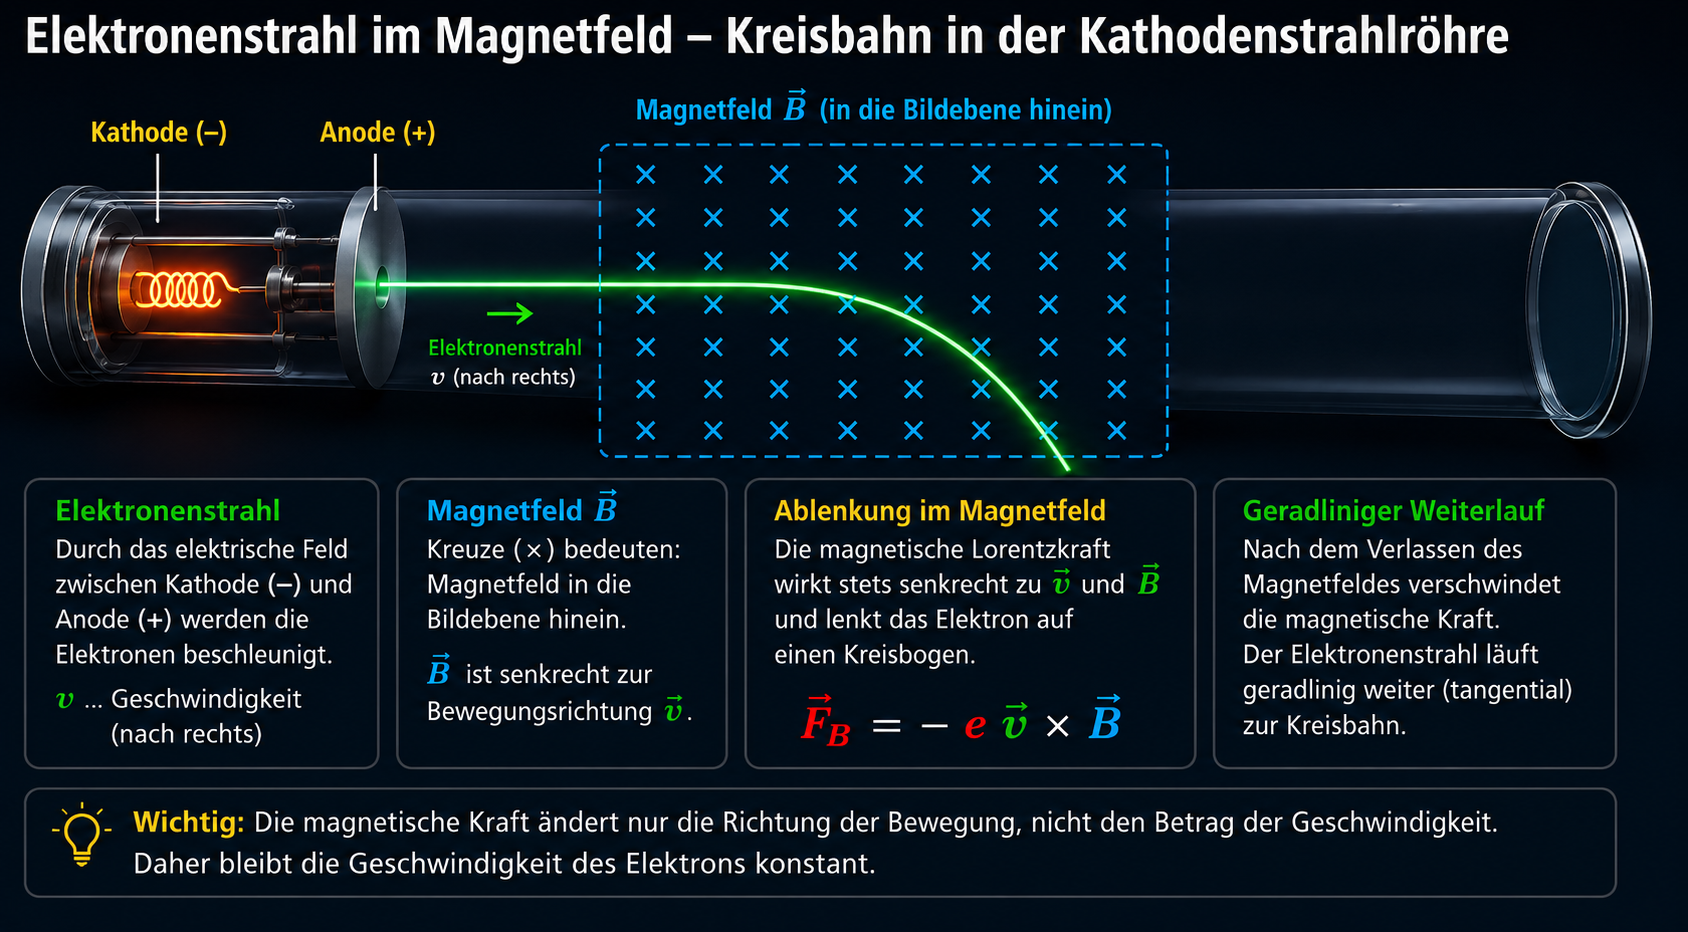
\includegraphics[width=\textwidth]{bilder/KathodenstrahlroehreKreisbahn.png}
\caption{Elektronenstrahl im Magnetfeld. Der Strahl wird zunächst durch das
	elektrische Feld zwischen Kathode und Anode beschleunigt. Im Magnetfeld, das
	in die Bildebene hinein zeigt, wirkt auf die bewegten Elektronen die
	magnetische Lorentzkraft. Diese Kraft steht stets senkrecht zur momentanen
	Geschwindigkeit und krümmt die Bahn des Strahls.}
\label{fig:elektronenstrahl-magnetfeld-kreisbahn}
\end{figure}

Wichtig ist dabei: Das Magnetfeld beschleunigt das Elektron nicht im Sinne
einer Energiezunahme. Es ändert nur die Richtung der Bewegung. Deshalb bleibt
der Betrag der Geschwindigkeit konstant, während sich die Bahn krümmt. Genau
dies unterscheidet die magnetische Ablenkung von der Ablenkung im elektrischen
Feld, bei der eine konstante seitliche Beschleunigung auftritt.